% !TeX root = Bericht_main.tex

\subsection{Aufgabe 27}
In dieser Aufgabe betrachten wir die Konvektions-Diffusions-Reaktions-Gleichung
\begin{align*}
  \partial_t c = \dive (\kappa_c \nabla c - cq) + r(c)
\end{align*}
im Gebiet $Mesh=Square500$. Dabei wird zum Zeitpunkt
$t=0$ eine Bakterienkolonie mit der Konzentration $c_0(x)$ platziert. Der Reaktionsterm $r(c)$ ist durch
\begin{align*}
  r(c) = Rc
\end{align*}
gegeben.
\subsubsection{Aufgabe 27.1}

\begin{figure}[H]
	\centering
	\captionabove{Verlauf der Masse und des Ausflusses
	(Konvektion = 1)}
	\subfigure[Reaction = -2.5]{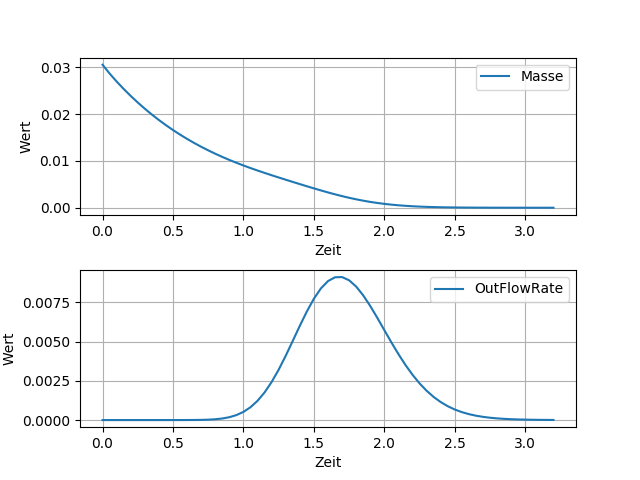
\includegraphics[width=0.32\textwidth]{../Aufgabe27/a/reaction=-2.5/plot.png}}
	\subfigure[Reaction = -1]{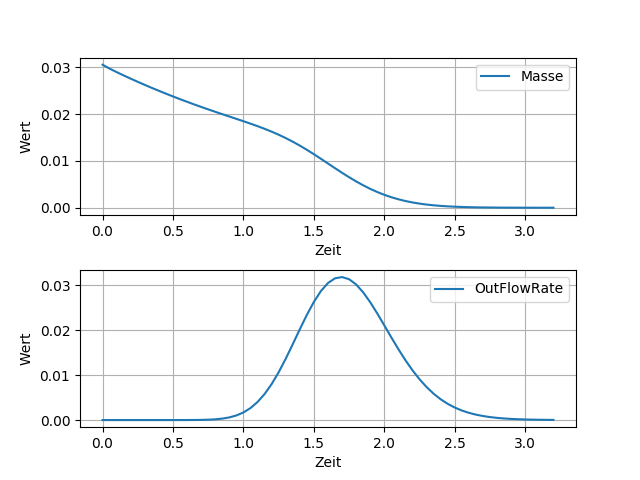
\includegraphics[width=0.32\textwidth]{../Aufgabe27/a/reaction=-1/plot.png}}
	\subfigure[Reaction = 0]{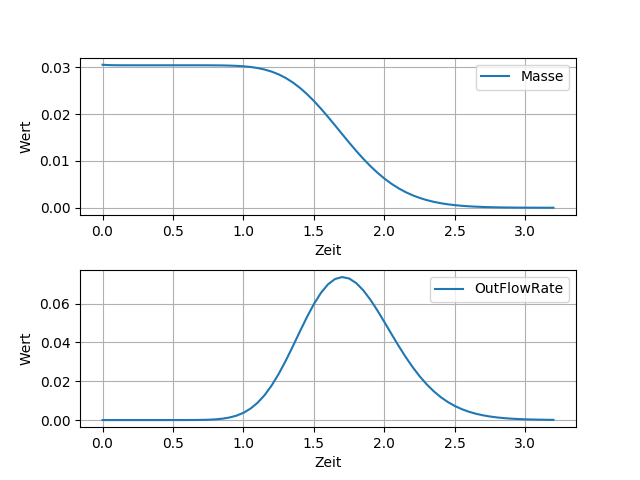
\includegraphics[width=0.32\textwidth]{../Aufgabe27/a/reaction=0/plot.png}}
	\subfigure[Reaction = 1]{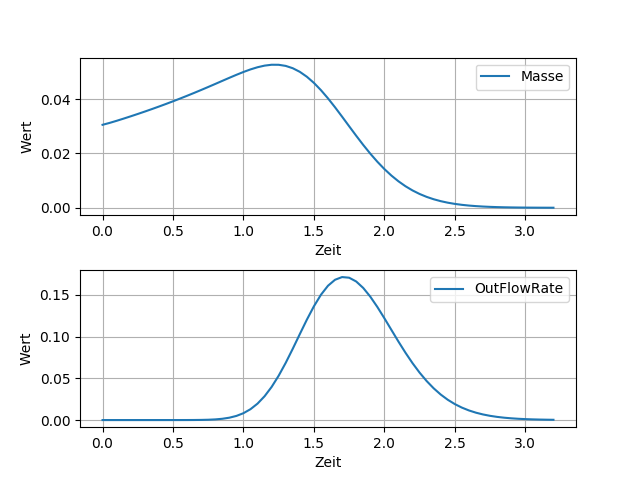
\includegraphics[width=0.32\textwidth]{../Aufgabe27/a/reaction=1/plot.png}}
	\subfigure[Reaction = 2.5]{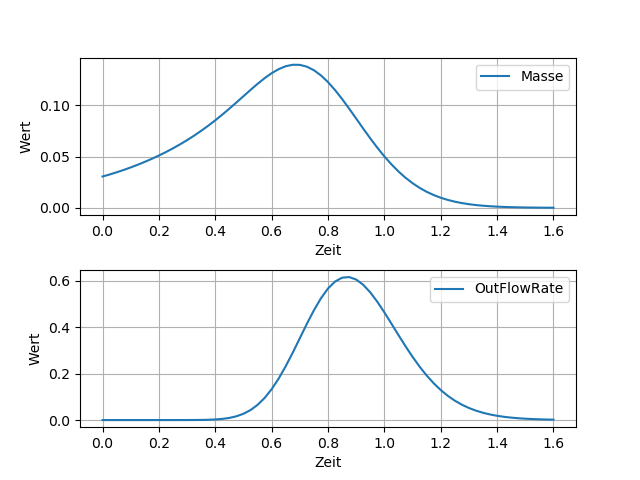
\includegraphics[width=0.32\textwidth]{../Aufgabe27/a/reaction=2.5/plot.png}}
	\subfigure[Reaction = 5]{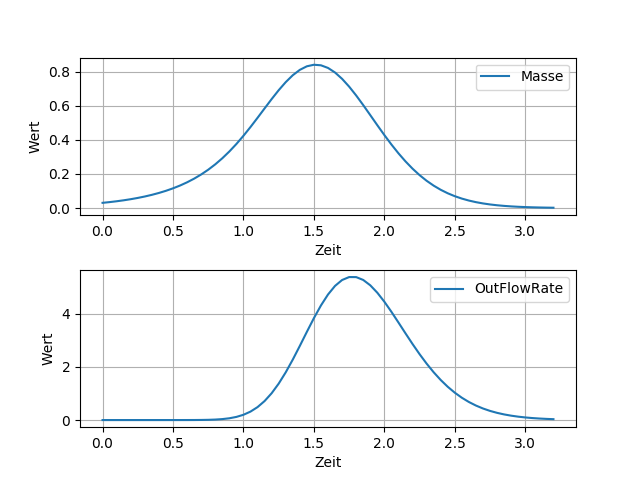
\includegraphics[width=0.32\textwidth]{../Aufgabe27/a/reaction=5/plot.png}}
\end{figure}

Anhand der Bilder erkennt man bei den negativen Reaktionsraten
den exponentiellen Zerfall der Masse, bei den positiven Reaktionsraten das exponentielle Wachstum der Masse bis zum Zeitpunkt $T=0.6$ sehr schön. Ab diesem Zeitpunkt überwiegt der Ausfluss des Fluids so stark, dass man den exponentiellen Verlauf nicht mehr beobachten kann.
Wird die Reaktion auf $0$ gesetzt erkennt man auch gut, dass sich die Konzentration der Bakterienkolonie nicht verändert und somit auch die Masse innerhalb des Gebietes bis zum Beginn des Ausflusses konstant bleibt.
Insgesamt bleibt außerdem festzuhalten, dass der Ausfluss nicht von der Reaktionsrate abhängt. 
Im Folgenden betrachten wir das Problem nochmals für eine niedrigere Konvektion:

\begin{figure}[H]
	\centering
	\captionabove{Verlauf der Masse und des Ausflusses (Konvektion = 0.1)}
	\subfigure[Reaction = 2.5]{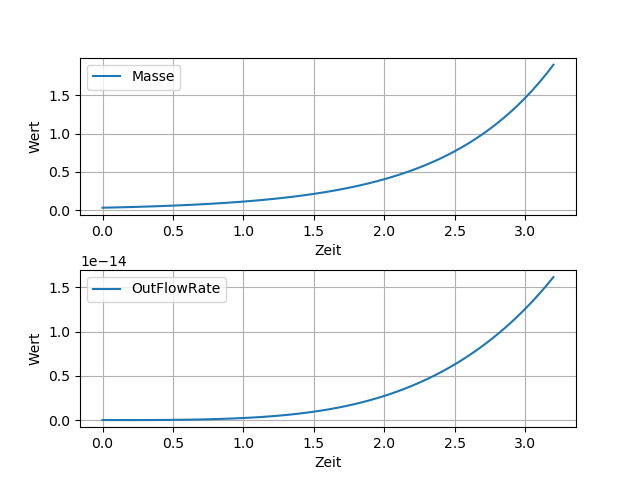
\includegraphics[width=0.8\textwidth]{../Aufgabe27/lowconvecreaction=2.5/plot.png}}
	\subfigure[$t=0$]{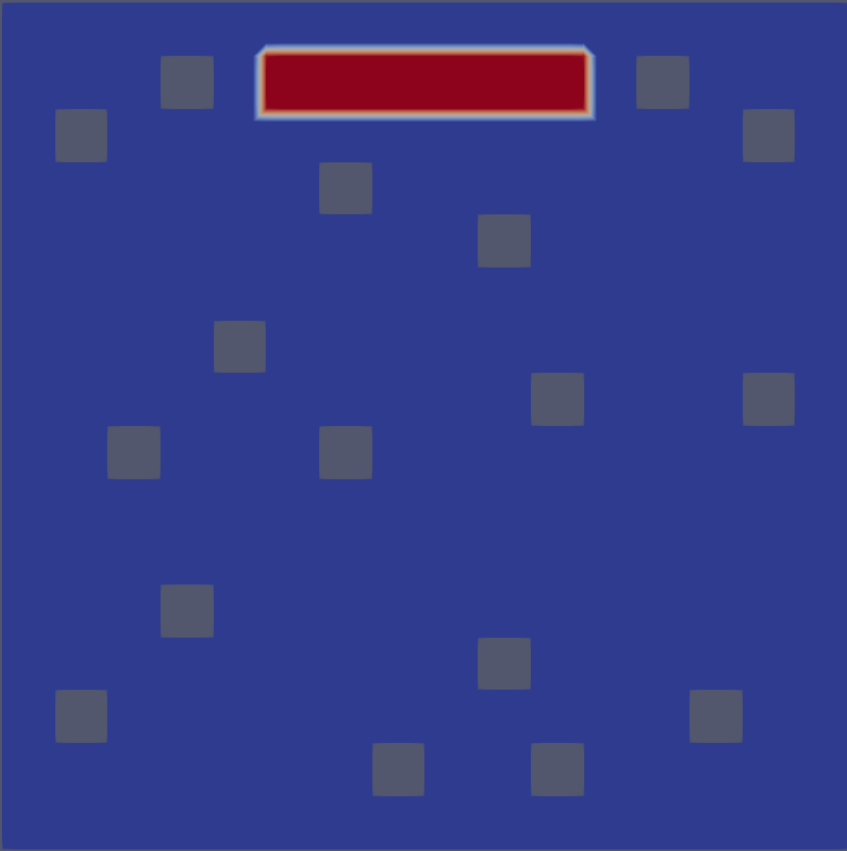
\includegraphics[width=0.32\textwidth]{../Aufgabe27/lowconvecreaction=2.5/animation0.png}}
	\subfigure[$t=0.5$]{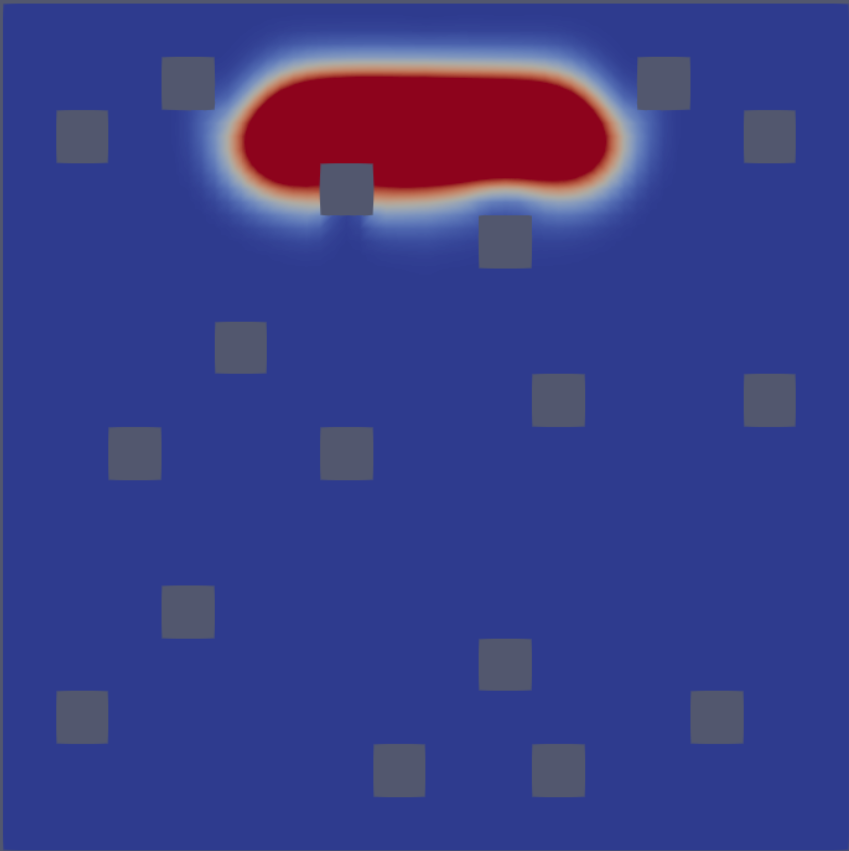
\includegraphics[width=0.32\textwidth]{../Aufgabe27/lowconvecreaction=2.5/animation20.png}}
	\subfigure[$t=1.6$]{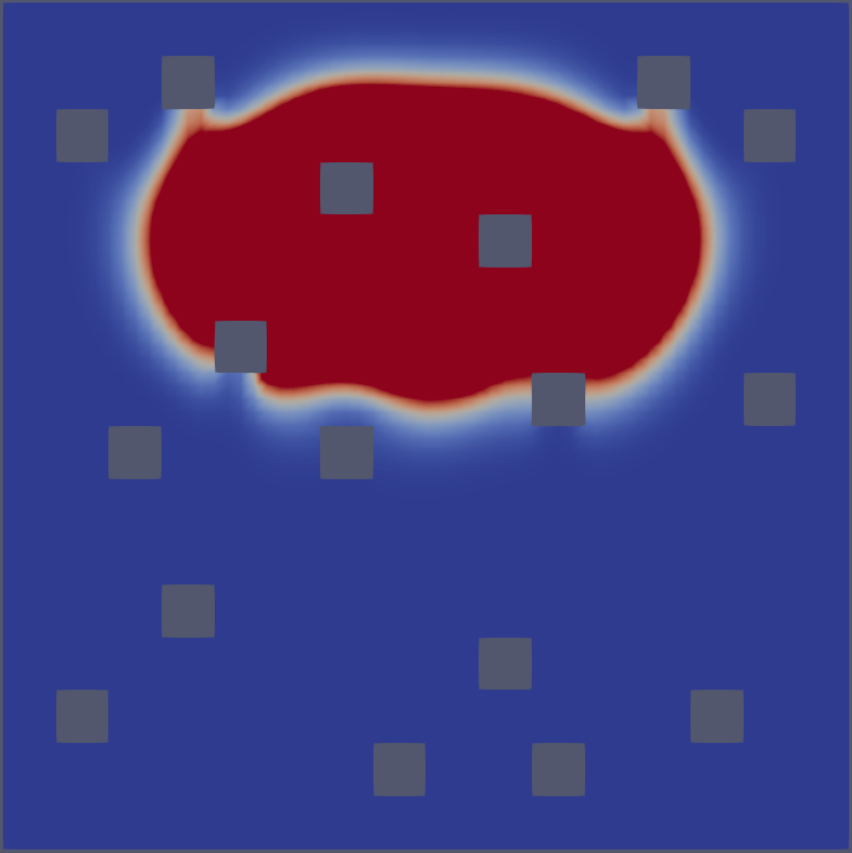
\includegraphics[width=0.32\textwidth]{../Aufgabe27/lowconvecreaction=2.5/animation64.png}}
\end{figure}
Anhand des Plots zum Endzeitpunkt erkennen wir, dass nun durch die niedrige Transportgeschwindigkeit das Fluid nicht ausfließt.
Dies erkennen wir auch am Verlauf der OutFlowRate über die Zeit, da die Werteskala hier im Bereich von $10^{-14}$ ist. Dadurch ergibt sich insgesamt ein schöner exponentieller Verlauf der Masse.
\subsubsection{Aufgabe 27.2}
In dieser Teilaufgabe untersuchen wir das Verhalten für immer kleiner werdende Diffusion. Wünschenswert wäre es hierbei, wie wir in der Vorlesung bereits analytisch gezeigt haben, dass wir uns immer weiter der Transportgleichung annähern. (Vergleiche dazu mit Theorieteil: Abschnitt \ref{Analyse für verschwindende Diffusion})

\begin{figure}[H]
	\centering
	\captionabove{Verlauf der Masse und des Ausflusses bei niedriger Diffusion \newline (Reaction = 0)}
	\subfigure[Diffusion = 0.0001]{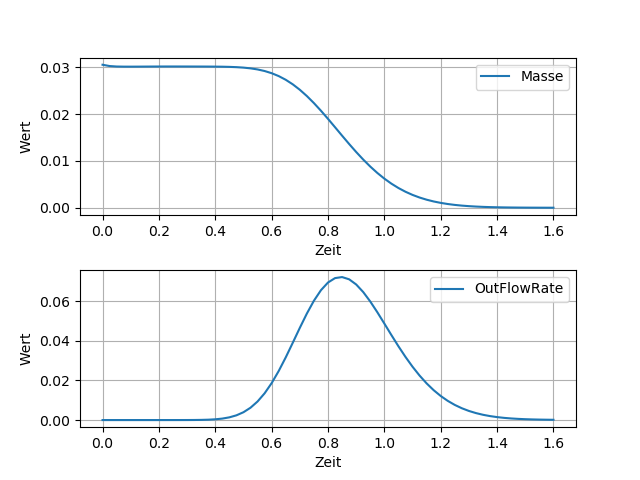
\includegraphics[width=0.32\textwidth]{../Aufgabe27/b/reaction=0_diffusion=0.0001/plot.png}}
	\subfigure[Diffusion = 0.00001]{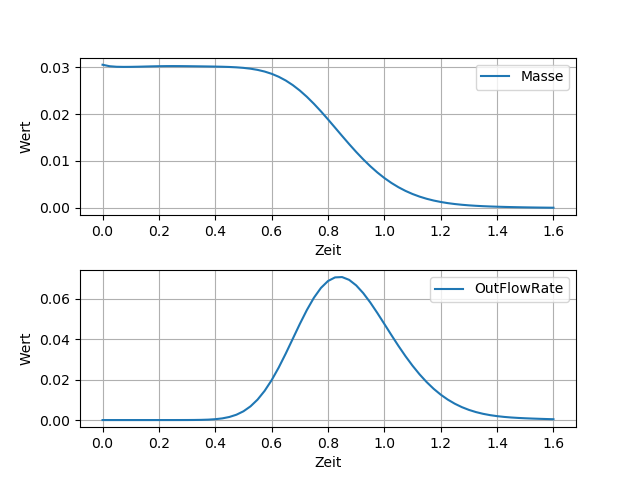
\includegraphics[width=0.32\textwidth]{../Aufgabe27/b/reaction=0_diffusion=1e-05/plot.png}}
	\subfigure[Diffusion = 0.000001]{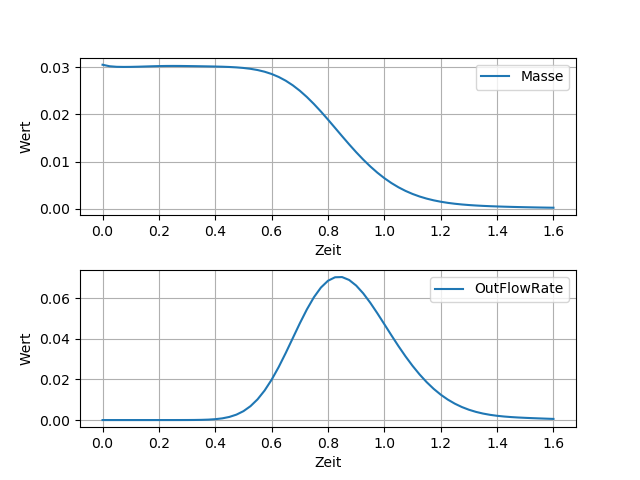
\includegraphics[width=0.32\textwidth]{../Aufgabe27/b/reaction=0_diffusion=1e-06/plot.png}}
\end{figure}

Zunächst betrachten wir hier die Verläufe für die Reaktionsrate $0$. Dabei fällt auf, dass hierbei bei kleiner werdender Diffusion so gut wie kein Unterschied zu erkennen ist. 

\begin{figure}[H]
	\centering
	\captionabove{Verlauf bei niedriger Diffusion = 0.000001}
	\subfigure[$t=0$]{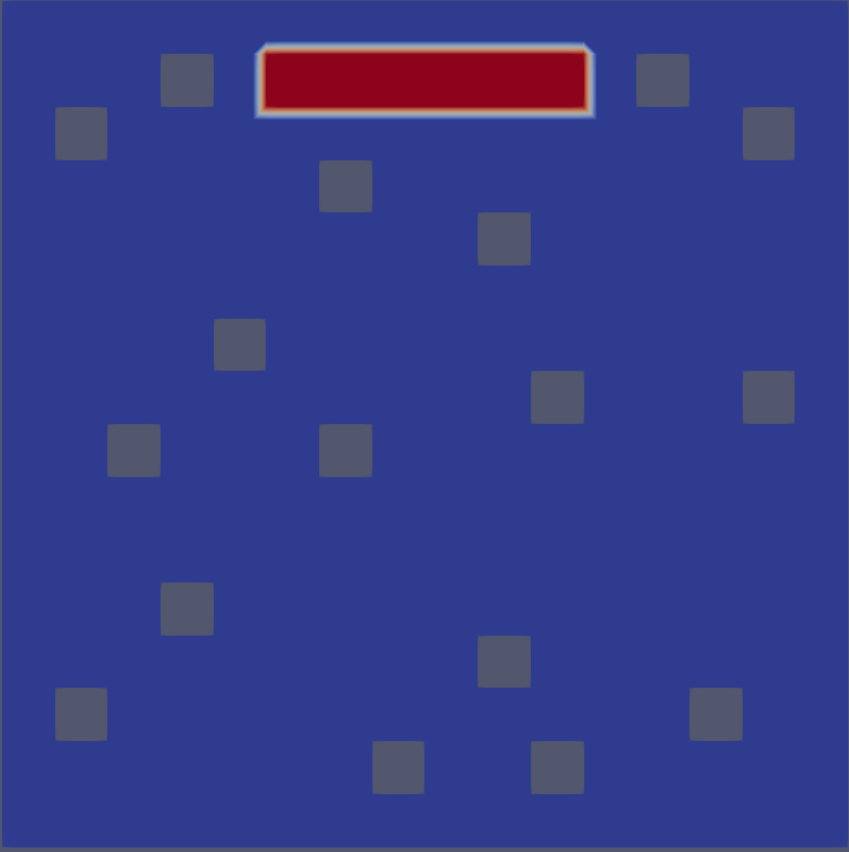
\includegraphics[width=0.32\textwidth]{../Aufgabe27/b/reaction=0_diffusion=1e-06/animation0.png}}
	\subfigure[$t=0.5$]{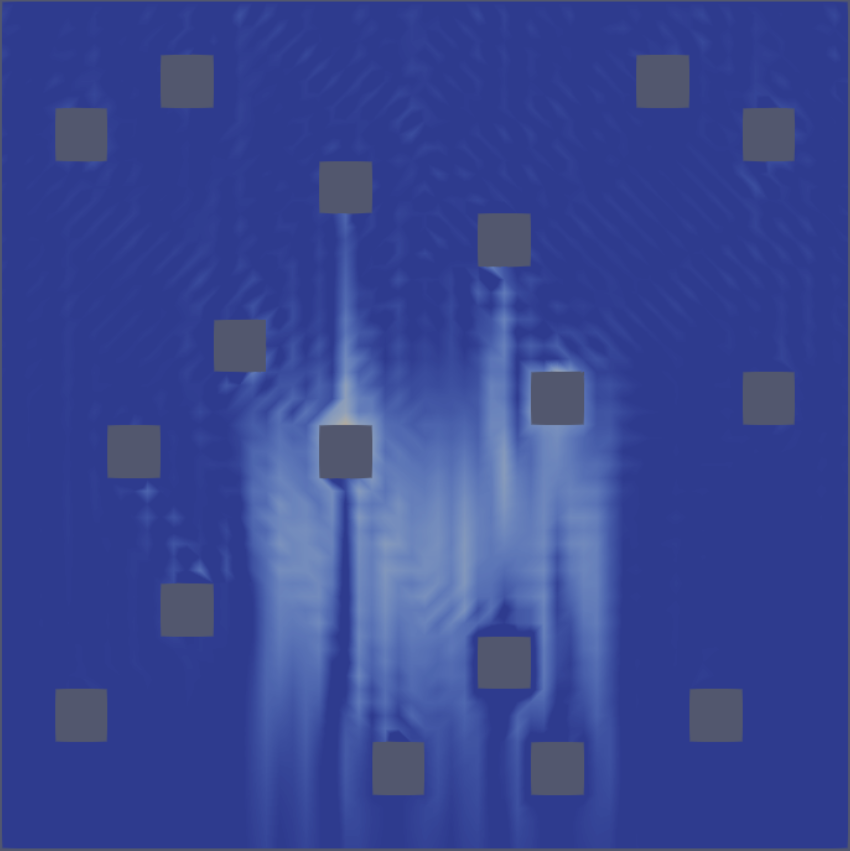
\includegraphics[width=0.32\textwidth]{../Aufgabe27/b/reaction=0_diffusion=1e-06/animation20.png}}
	\subfigure[$t=1$]{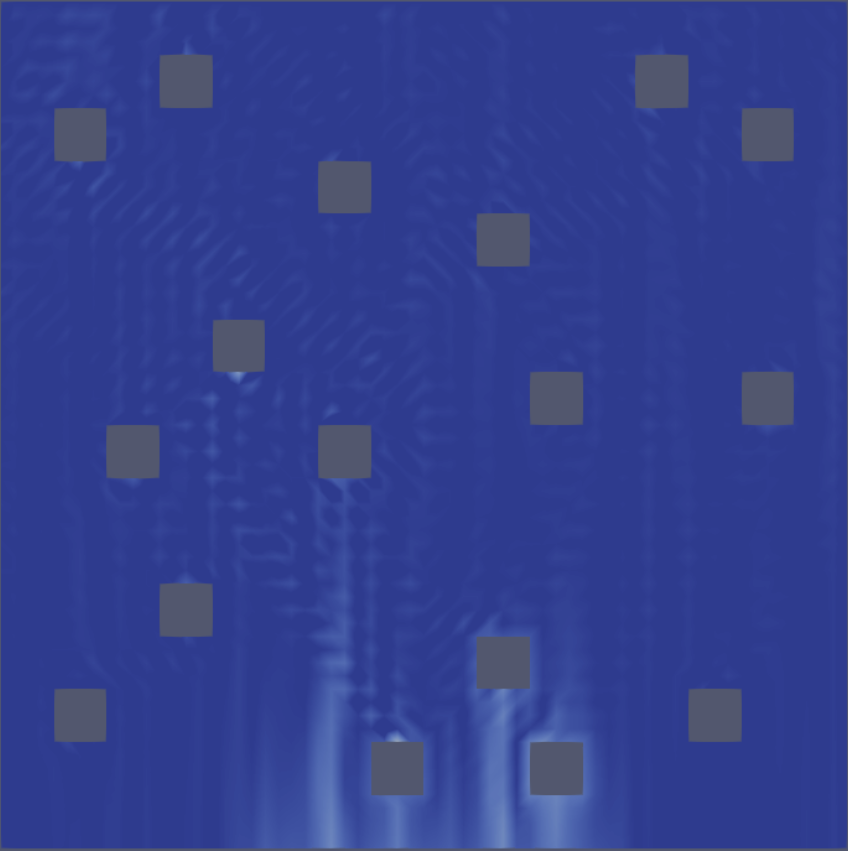
\includegraphics[width=0.32\textwidth]{../Aufgabe27/b/reaction=0_diffusion=1e-06/animation40.png}}
\end{figure}

Anhand der zugehörigen Lösungsplots lassen sich allerdings leichte Oszillationen der Lösung erkennen. Diese fallen für die Reaktionsrate $0$ aber noch so gering aus, dass es sich nicht in dem Masseverlauf wiederspiegelt.

\begin{figure}[H]
	\centering
	\captionabove{Verlauf der Masse und des Ausflusses bei niedriger Diffusion \newline (Reaction = 5)}
	\subfigure[Diffusion = 0.0001]{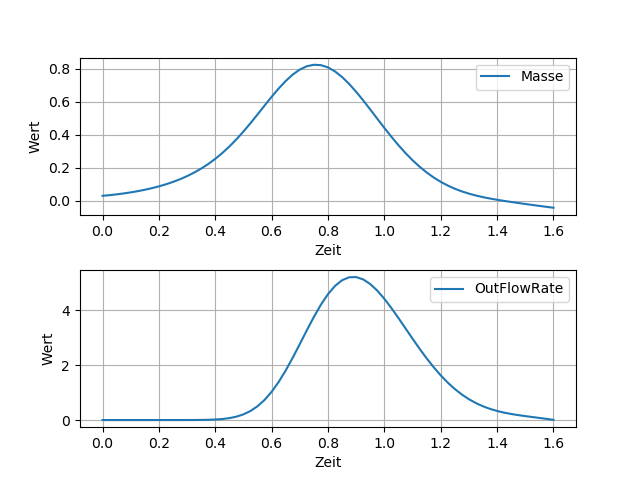
\includegraphics[width=0.32\textwidth]{../Aufgabe27/b/reaction=5_diffusion=0.0001/plot.png}}
	\subfigure[Diffusion = 0.00001]{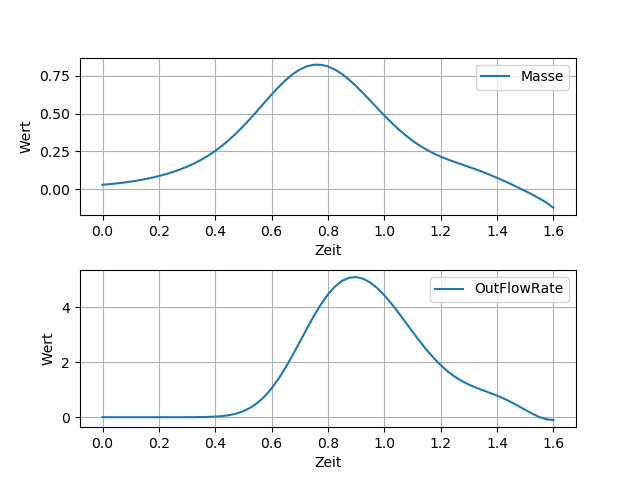
\includegraphics[width=0.32\textwidth]{../Aufgabe27/b/reaction=5_diffusion=1e-05/plot.png}}
	\subfigure[Diffusion = 0.000001]{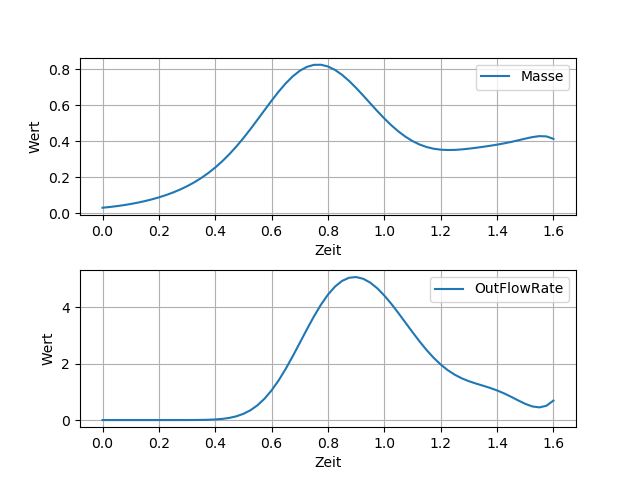
\includegraphics[width=0.32\textwidth]{../Aufgabe27/b/reaction=5_diffusion=1e-06/plot.png}}
\end{figure}

Betrachten wir nun die Verläufe mit der Reaktionsrate $5$. Für die größte Diffusion $(0.0001)$ erhalten wir hier noch den zu erwartenden Verlauf. Allerdings ergeben sich bei den niedrigeren Diffusionswerten erhebliche Probleme. Sowohl beim Ausfluss, als auch bei der Masse bekommen wir eine große Abweichung im Vergleich zur Diffusion $0.0001$. Der Grund dafür wird anhand der folgenden Plots deutlich:

\begin{figure}[H]
	\centering
	\captionabove{Verlauf bei niedriger Diffusion 0.000001}
	\subfigure[$t=0$]{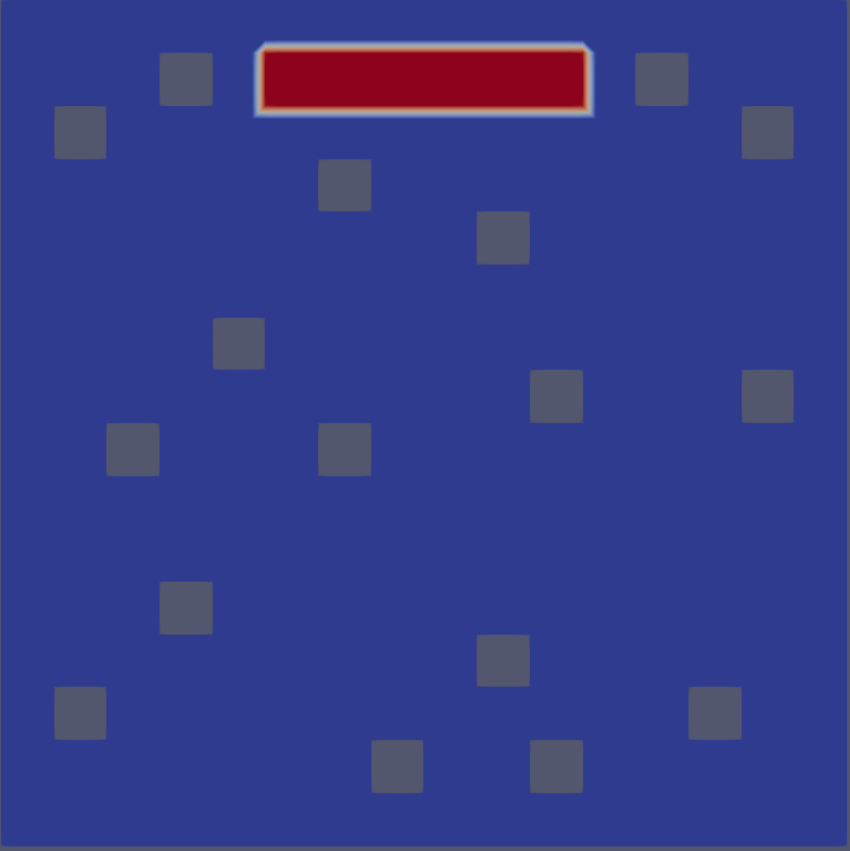
\includegraphics[width=0.40\textwidth]{../Aufgabe27/b/reaction=5_diffusion=1e-06/animation0.png}}
	\subfigure[$t=0.5$]{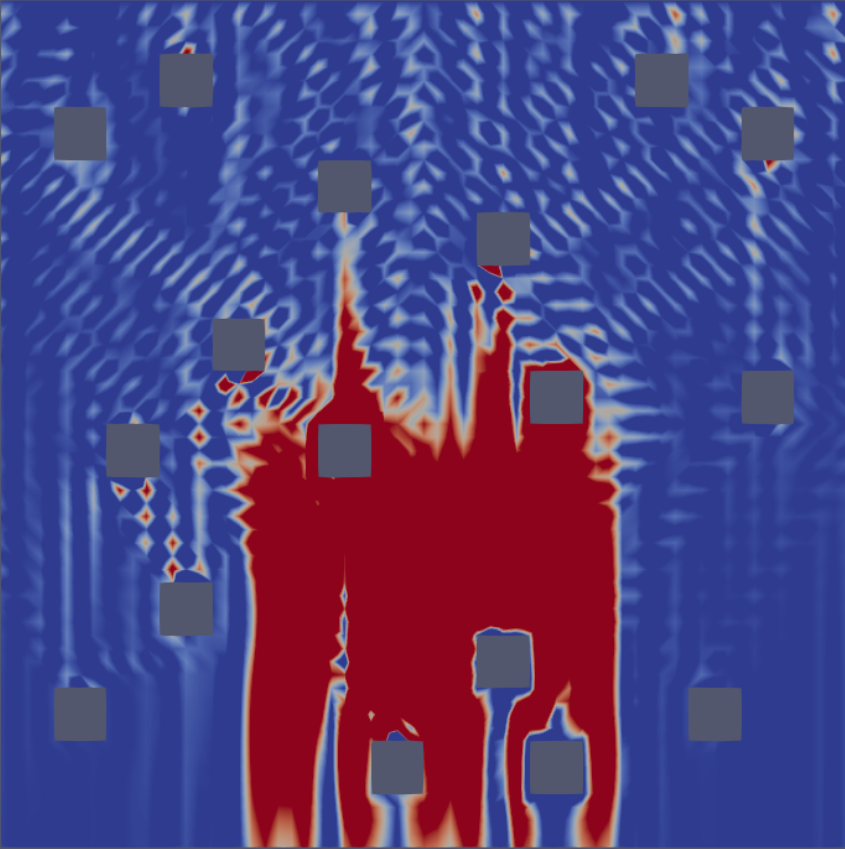
\includegraphics[width=0.40\textwidth]{../Aufgabe27/b/reaction=5_diffusion=1e-06/animation20.png}}
	\subfigure[$t=1.0$]{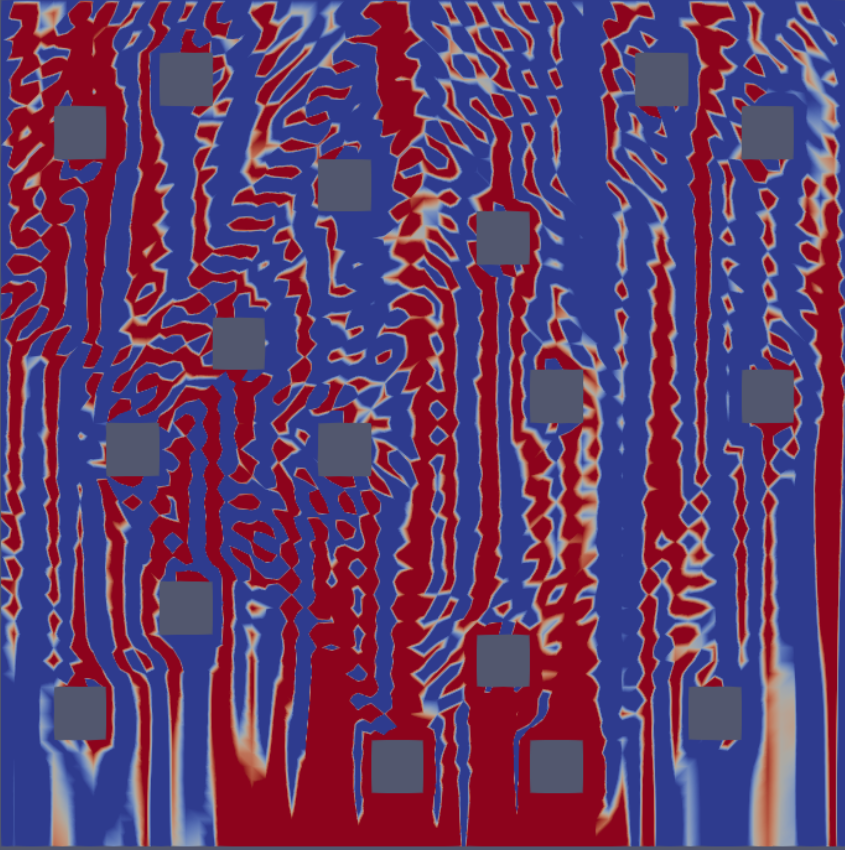
\includegraphics[width=0.40\textwidth]{../Aufgabe27/b/reaction=5_diffusion=1e-06/animation40.png}}
	\subfigure[$t=1.6$]{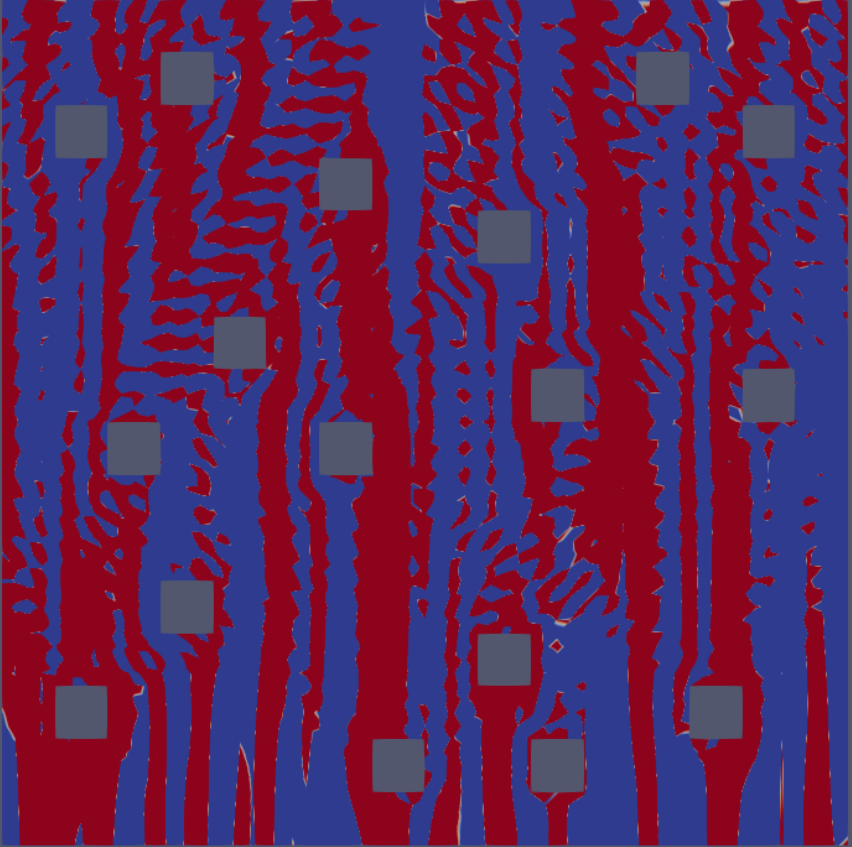
\includegraphics[width=0.405\textwidth]{../Aufgabe27/b/reaction=5_diffusion=1e-06/animation64.png}}
\end{figure}

Hieran sehen wir, dass die Lösung bereits zum Zeitpunkt $t=0.5$
erhebliche Oszillationen hat. Zu späteren Zeitpunkten lässt sich keinerlei Bezug zu vorherigen Zeitpunkten herstellen. Dies ist der Tatsache geschuldet, dass sich unser bisheriges Verfahren, die klassische Finite Elemente Methode (FEM), nicht zum Lösen der Konvektions-Diffusions-Reaktions-Gleichung für niedrige Diffusion eignet, da die so entstehende Lösung sehr stark von der erwarteten Lösung abweicht (Vergleiche dazu mit Theorieteil: Abschnitt \ref{Analyse für verschwindende Diffusion}) .
Unser Ziel in den nächsten Aufgaben (27.3 und 32) besteht nun unter anderem darin, dass wir ein Verfahren finden, welches dieses Problem löst.

\subsubsection{Aufgabe 27.3}
In dieser Teilaufgabe verwenden wir nun, anders als zuvor mit linearen Ansatzelementen, quadratische Ansatzelemente (serendipity) auf den Dreiecken des Gitters. Hierbei untersuchen wir die Lösungsqualität des Verfahrens in Bezug auf eine geringe Diffusion (Grenzfall $\to$ 0). Dabei werden wir dieses Problem für unterschiedliche Gitterweiten betrachten.
Zuerst schauen wir uns die Massen- und Ausflussverläufe für die Reaktionsrate $5$ auf Level 2 und 3 an:
\begin{figure}[H]
	\centering
	\captionabove{Verlauf der Masse und des Ausflusses bei niedriger Diffusion}
	\subfigure[Level=2, Diffusion=0.0001]{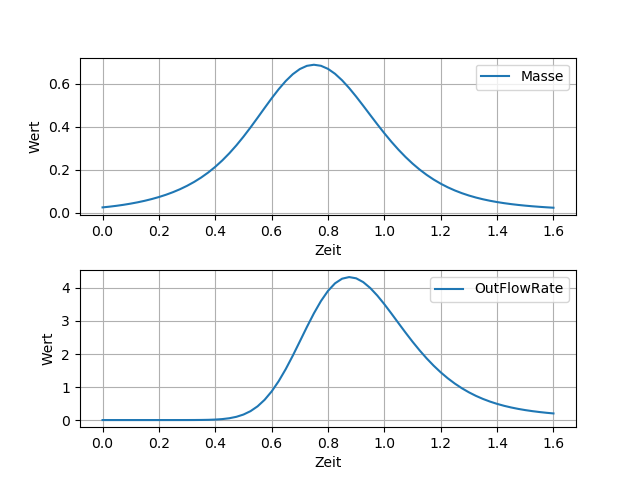
\includegraphics[width=0.32\textwidth]{../Aufgabe27/c/serendipity_lvl=2_reaction=5_diffusion=0.0001/plot.png}}
	\subfigure[Level=2, Diffusion=0.00001]{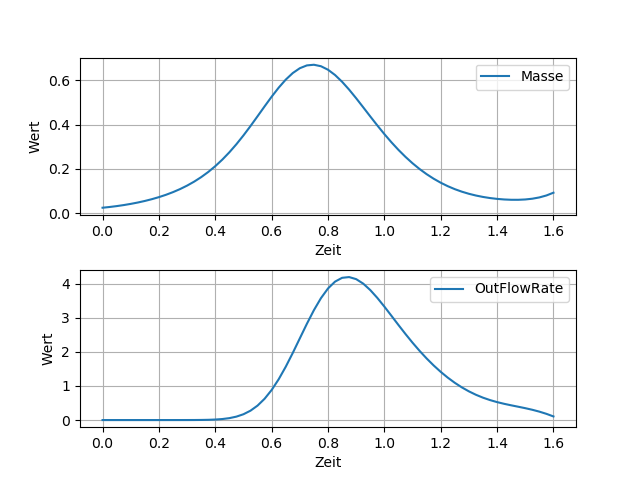
\includegraphics[width=0.32\textwidth]{../Aufgabe27/c/serendipity_lvl=2_reaction=5_diffusion=1e-05/plot.png}}
	\subfigure[Level=2, Diffusion=0.000001]{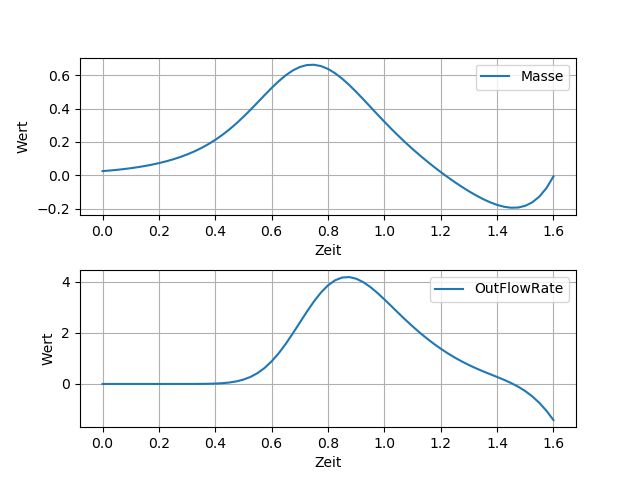
\includegraphics[width=0.32\textwidth]{../Aufgabe27/c/serendipity_lvl=2_reaction=5_diffusion=1e-06/plot.png}}
	\subfigure[Level=3, Diffusion=0.0001]{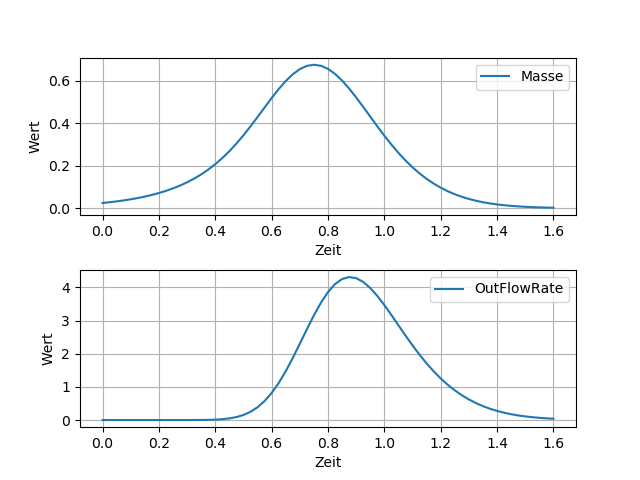
\includegraphics[width=0.32\textwidth]{../Aufgabe27/c/serendipity_lvl=3_reaction=5_diffusion=0.0001/plot.png}}
	\subfigure[Level=3, Diffusion=0.00001]{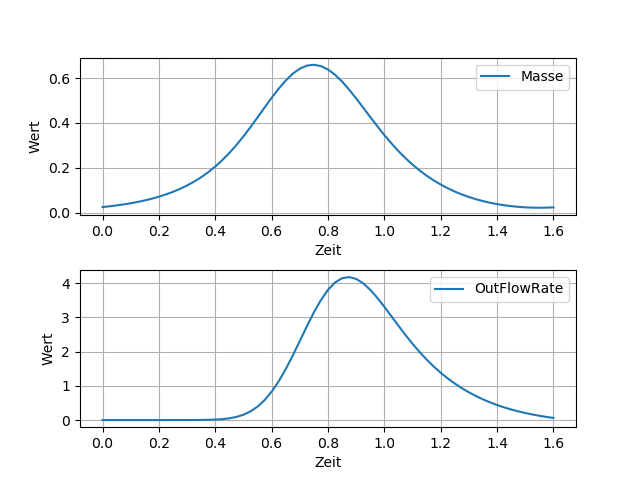
\includegraphics[width=0.32\textwidth]{../Aufgabe27/c/serendipity_lvl=3_reaction=5_diffusion=1e-05/plot.png}}
	\subfigure[Level=3, Diffusion=0.000001]{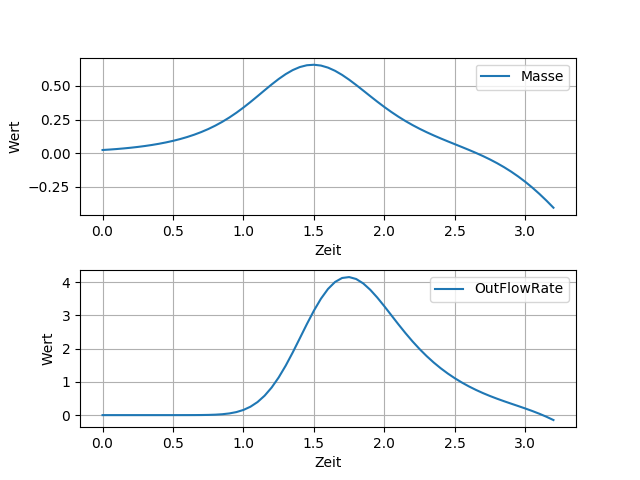
\includegraphics[width=0.32\textwidth]{../Aufgabe27/c/serendipity_lvl=3_reaction=5_diffusion=1e-06/plot.png}}
\end{figure}

Hierbei löst unser Verfahren für beide Level die Diffusion 0.0001 gut. Bei Level 2 erhalten wir aber, im Gegensatz zum Level 3, bereits wieder Oszillationen. Dadurch können wir festhalten, dass man durch die Halbierung der Gitterweite dem Problem entgegen wirken kann. Bei der kleinsten Diffusion sind aber trotzdem bei beiden Levels große Probleme festzustellen.

Im Folgenden vergleichen wir die Lösungsplots der FEM mit linearen Ansatzelementen auf Level 2 mit dem serendipity Verfahren (quadratische Ansatzelemente auf Dreiecken) auf Level 2 und 3:
 
\begin{figure}[H]
	\centering
	\captionabove{Verlauf bei Diffusion 0.00001 (FEM)}
	\subfigure[$t=0$]{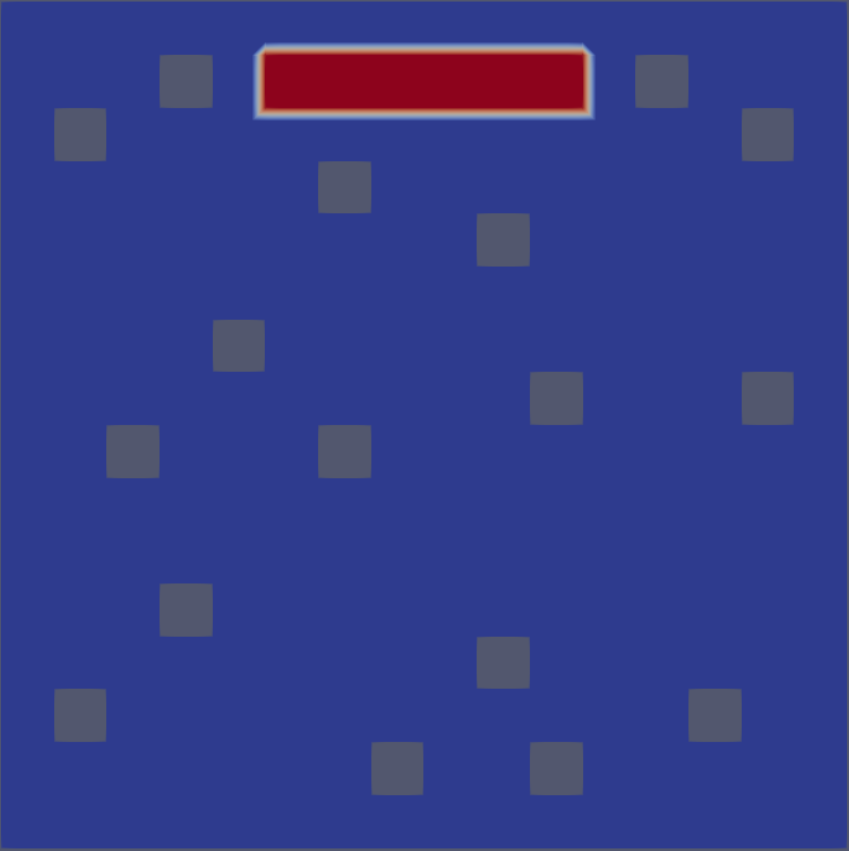
\includegraphics[width=0.32\textwidth]{../Aufgabe27/b/reaction=5_diffusion=1e-05/animation0.png}}
	\subfigure[$t=0.5$]{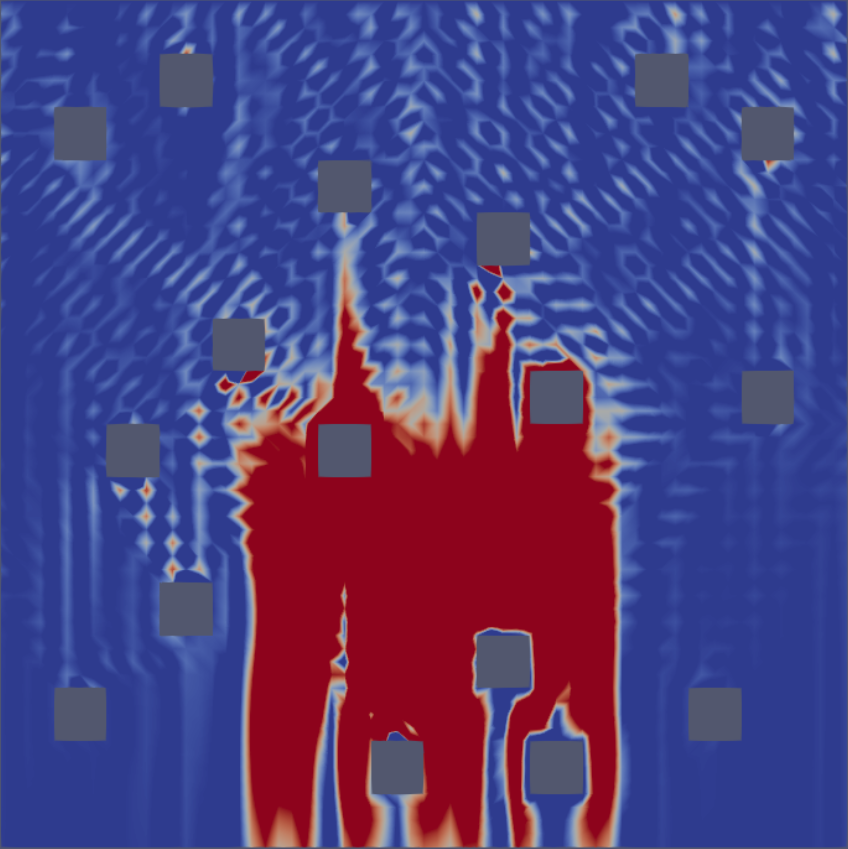
\includegraphics[width=0.32\textwidth]{../Aufgabe27/b/reaction=5_diffusion=1e-05/animation20.png}}
	\subfigure[$t=1.0$]{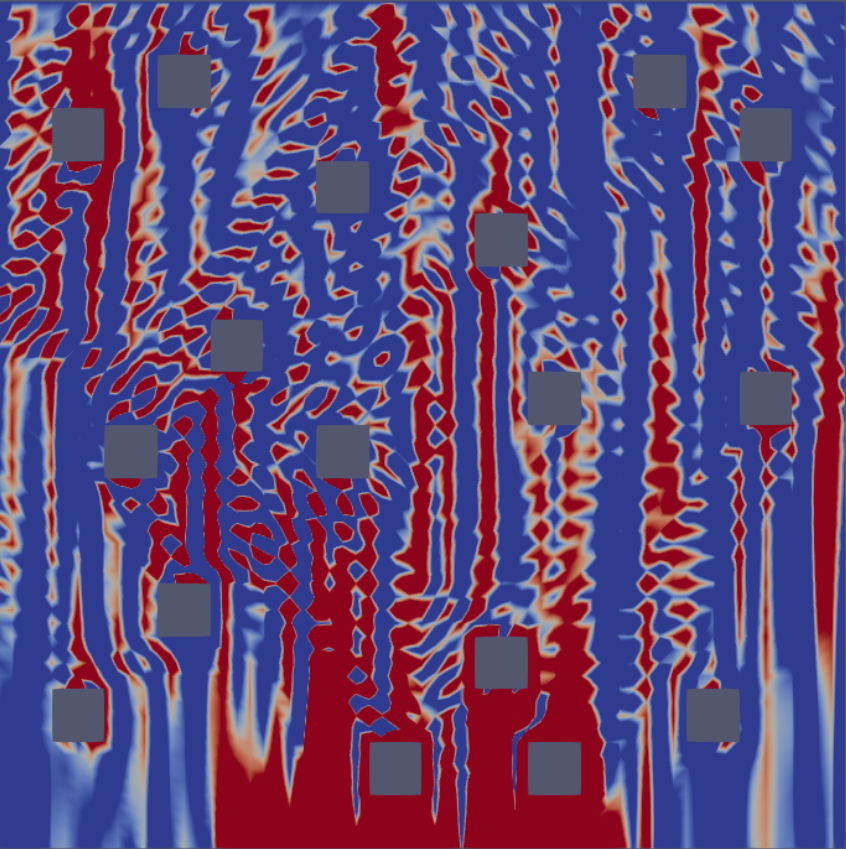
\includegraphics[width=0.32\textwidth]{../Aufgabe27/b/reaction=5_diffusion=1e-05/animation40.png}}
\end{figure}

\begin{figure}[H]
	\centering
	\captionabove{Verlauf bei Diffusion 0.00001 (serendipity lvl 2)}
	\subfigure[$t=0$]{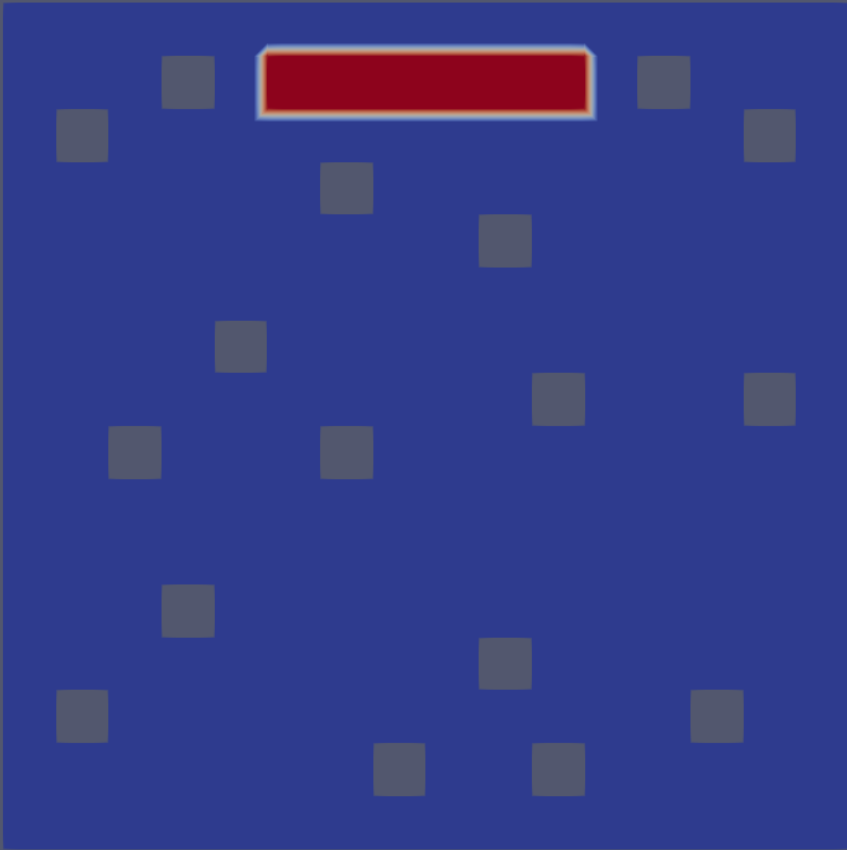
\includegraphics[width=0.32\textwidth]{../Aufgabe27/c/serendipity_lvl=2_reaction=5_diffusion=1e-05/animation0.png}}
	\subfigure[$t=0.5$]{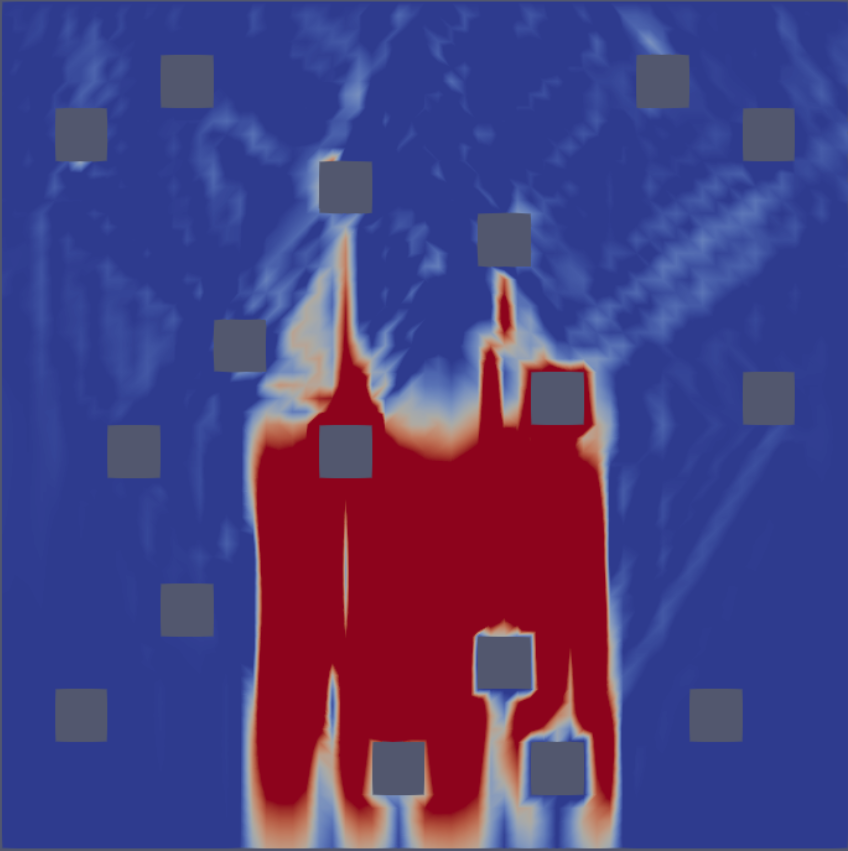
\includegraphics[width=0.32\textwidth]{../Aufgabe27/c/serendipity_lvl=2_reaction=5_diffusion=1e-05/animation20.png}}
	\subfigure[$t=1.0$]{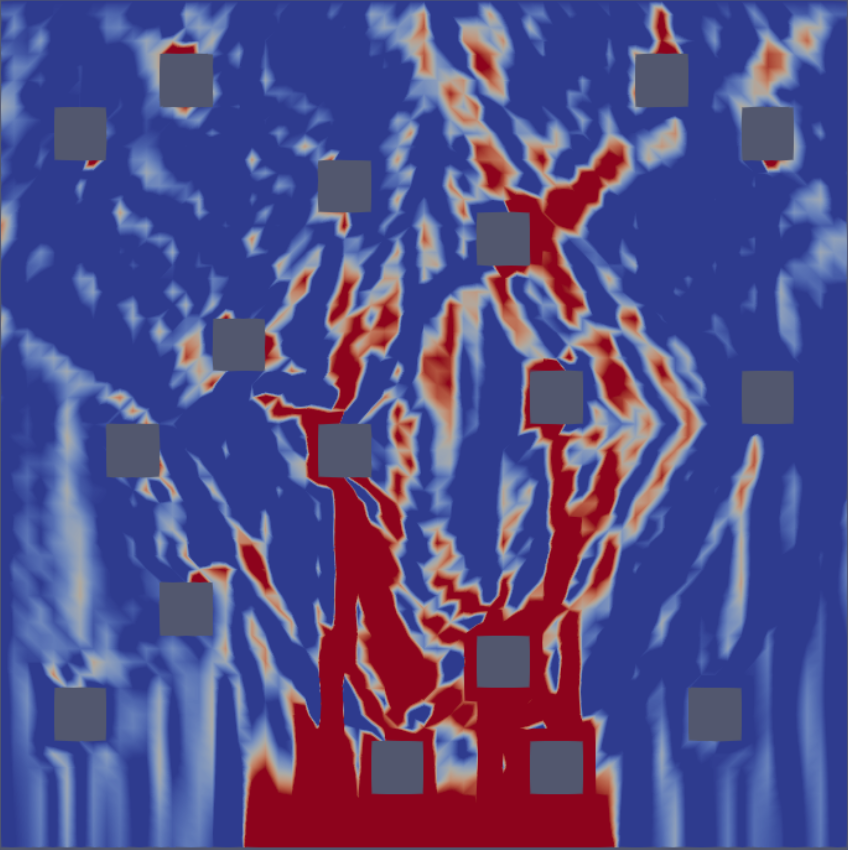
\includegraphics[width=0.32\textwidth]{../Aufgabe27/c/serendipity_lvl=2_reaction=5_diffusion=1e-05/animation40.png}}
\end{figure}

\begin{figure}[H]
	\centering
	\captionabove{Verlauf bei Diffusion 0.00001 (serendipity lvl 3)}
	\subfigure[$t=0$]{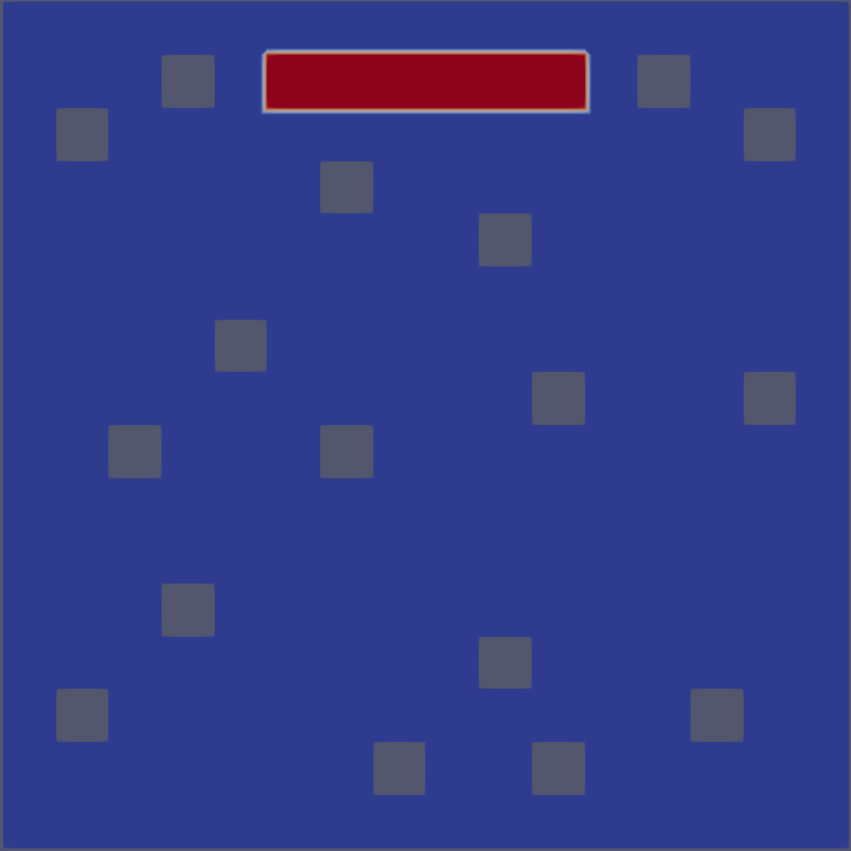
\includegraphics[width=0.32\textwidth]{../Aufgabe27/c/serendipity_lvl=3_reaction=5_diffusion=1e-05/animation0.png}}
	\subfigure[$t=0.5$]{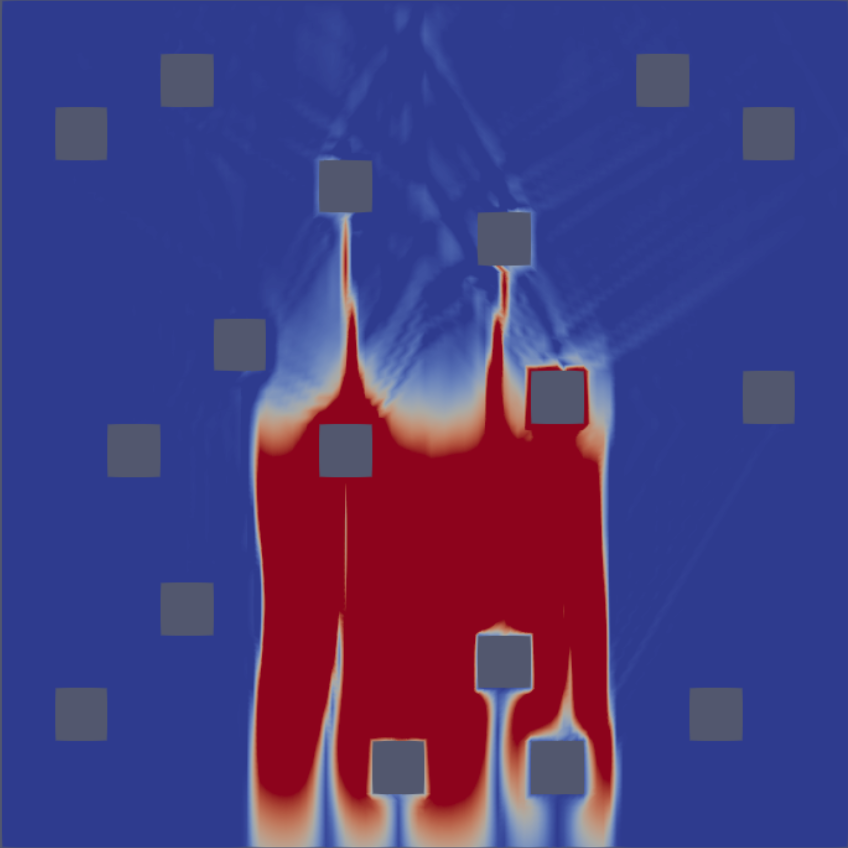
\includegraphics[width=0.32\textwidth]{../Aufgabe27/c/serendipity_lvl=3_reaction=5_diffusion=1e-05/animation20.png}}
	\subfigure[$t=1.0$]{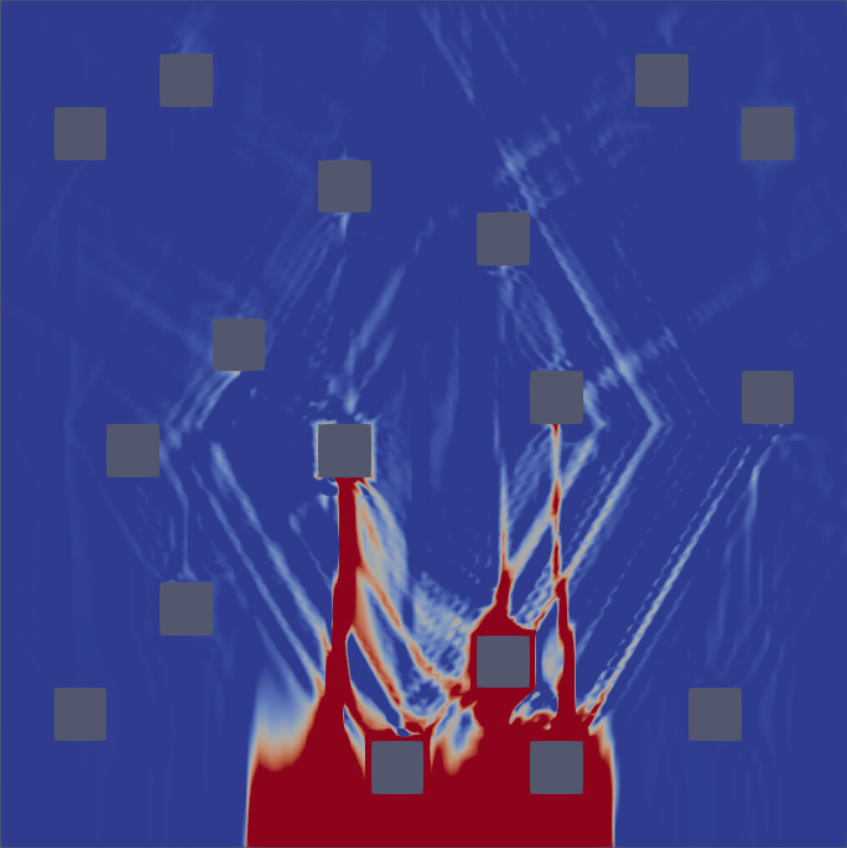
\includegraphics[width=0.32\textwidth]{../Aufgabe27/c/serendipity_lvl=3_reaction=5_diffusion=1e-05/animation40.png}}
\end{figure}

An den Lösungsplots erkennen wir, dass das serendipity Verfahren auf gleichem Level zum Zeitpunkt $t=0.5$ etwas besser ist, da es weniger Oszillationen hat. Allerdings wird auch anhand des Zeitpunktes $t=1.0$ deutlich, dass das Verfahren trotzdem mit der Zeit immer mehr Oszillationen entwickelt und somit unbrauchbar ist.
Auf Level 3 ist das serendipity Verfahren hingegen für diese Diffusion noch geeignet. Insgesamt erhalten wir damit durch die quadratischen Ansatzelemente einen etwas besseren Löser als mit linearen Ansatzelementen.



